\documentclass[onecolumn, draftclsnofoot,10pt, compsoc]{IEEEtran}
\usepackage[utf8]{inputenc}
\usepackage{graphicx}
\graphicspath{ {./} }
\usepackage{caption}
\usepackage{url}
\usepackage{setspace}
\usepackage{parskip}
\usepackage[table,xcdraw]{xcolor}
\usepackage{geometry}
\usepackage{tabularx}
\geometry{textheight=9.5in, textwidth=7in}

% 1. Fill in these details
\title{Group 73: Virtual Reality Printing}
\author{Stephen Hoffmann, Stewart Rodger, Nicholas Pugliese, Kyle Tyler, Symon Ramos}
\date{November 2018}
\def \CapstoneTeamName{		    Group 73: Virtual Reality Printing }
\def \CapstoneTeamNumber{		73}
\def \GroupMemberOne{			Symon Ramos}
\def \GroupMemberTwo{			Stephen Hoffman}
\def \GroupMemberThree{			Nicholas Pugliese}
\def \GroupMemberFour{			Stewart Rodger}
\def \GroupMemberFive{			Kyle Tyler}
\def \CapstoneProjectName{		Developing Virtual Reality Based Training Experiences for HP's PageWide Web Press Product Line}
\def \CapstoneSponsorCompany{	HP Inc}
\def \CapstoneSponsorPerson{		Tim Holt}



% 2. Uncomment the appropriate line below so that the document type works
\def \DocType{		
				Design Document Revision 2
				%Progress Report
				}
			
\newcommand{\NameSigPair}[1]{\par
\makebox[2.75in][r]{#1} \hfil 	\makebox[3.25in]{\makebox[2.25in]{\hrulefill} \hfill		\makebox[.75in]{\hrulefill}}
\par\vspace{-12pt} \textit{\tiny\noindent
\makebox[2.75in]{} \hfil		\makebox[3.25in]{\makebox[2.25in][r]{Signature} \hfill	\makebox[.75in][r]{Date}}}}
% 3. If the document is not to be signed, uncomment the RENEWcommand below
%\renewcommand{\NameSigPair}[1]{#1}

%%%%%%%%%%%%%%%%%%%%%%%%%%%%%%%%%%%%%%%
\begin{document}
\maketitle
    \begin{abstract}
        Proposed is a training program capable of providing the same level of training from a remote location away from real HP printer technology by the use of a virtual reality simulations. The program will contain several different modes and scenarios to be used in place of actual training on the HP facility.
    \end{abstract}
\newpage
\pagenumbering{arabic}
\tableofcontents
% 7. uncomment this (if applicable). Consider adding a page break.
%\listoffigures
%\listoftables

\section*{Revisions}

\begin{table}[ht!]
\begin{tabularx}{\textwidth}{|l|X|X|}
\hline
\rowcolor[HTML]{C0C0C0} 
Section & Original & New \\ \hline
Scope &     The software to be produced is to be called Web Press VR. This software product will allow users to learn how to use
an HP PageWide Web Press in a completely virtual environment. Users will be able to use a Web Press virtually in a
sandbox mode, a full training mode, and specific skill training modules. Letting users explore a Web Press in a sand
box mode will give the user familiarity with the Web Press that will carry over into the real world. A full training mode
will allow users to see what it is like to use a Web Press, from the beginning to the end of an operation cycle. The skill
training modules will allow users to familiarize themselves with specific tasks and operations one may wish to perform
with a Web Press.     &   The software to be produced is to be called Web Press VR. This software product will allow users to learn how to use
an HP PageWide Web Press in a completely virtual environment. Users will be able to use a Web Press virtually in a
sandbox mode, a full training mode, and specific skill training modules. Letting users explore a Web Press in a sand
box mode will give the user familiarity with the Web Press that will carry over into the real world. A full training mode
will allow users to see what it is like to use a Web Press, from the beginning to the end of an operation cycle. The skill
training modules will allow users to familiarize themselves with specific tasks and operations one may wish to perform
with a Web Press. Our goal is to facilitate the creation of a program, and to construct a prototype that can be shown off as a feasibility test to management at HP. This prototype will serve to create the conversation that money should be spent internally at HP to develop the VR program further.  \\ \hline
\end{tabularx}
\end{table}

\clearpage



% 8. now you write!

\section{Overview}
\subsection{Scope}
The software to be produced is to be called Web Press VR. This software product will allow users to learn how to use an HP PageWide Web Press in a completely virtual environment. Users will be able to use a Web Press virtually in a sandbox mode, a full training mode, and specific skill training modules. Letting users explore a Web Press in a sand box mode will give the user familiarity with the Web Press that will carry over into the real world. A full training mode will allow users to see what it is like to use a Web Press, from the beginning to the end of an operation cycle. The skill training modules will allow users to familiarize themselves with specific tasks and operations one may wish to perform with a Web Press.

The benefits of using virtual reality to train people to use the Web Press are reductions in training costs, reductions in time required to train, and increases in total understanding of the system. An ultimate goal of the system is to streamline to whole training process, and to serve as a viable alternative to in-person training. We aim to show that virtual reality is an invaluable training tool, and has uses beyond just the scope of this particular product. Our goal is to facilitate the creation of a program, and to construct a prototype that can be shown off as a feasibility test to management at HP. This prototype will serve to create the conversation that money should be spent internally at HP to develop the VR program further.
\subsection{Purpose}
The purpose of our software is to be a virtual reality training application to work with modern virtual reality headsets. By taking advantage of the increased accessibility of virtual reality as well as the decreased cost of hardware, we hope to build an application that will reduce the costs associated with training people to use HP's PageWide Web Press product line. Developing these training scenarios will improve the effectiveness of HP's current training procedure as well as mitigate the costs and risks of handling real machinery by the trainees.
\subsection{Intended Audience}
The intended audience of our software will ultimately be personnel who are enrolled to be trained on HP's PageWide Web Press product line, whether it be HP employees or customers who have purchased the technology. Teachers and supervisors of the training program of HP would also be involved in the utilization of our software. Relative to the scope of our project, we intend for our software to be reviewed in-depth by our client and any other potential personnel that our client recommends. Our client will use our software as an additional means to prompt upper management of HP to invest and allocate more resources into the development of VR software that trains personnel on PageWide Web Press use. 
\subsection{Conformance}
The ultimate goal of the VR system is to provide an environment that allows the user to receive the same quality of training as if they were participating in an in-person training event at an actual HP PageWide Web Press location.

\section{Definitions}
\begin{enumerate}
    \item Virtual Reality (VR) - A simulated computer environment that immerses the user in a 3D space
    \item PageWide Web Press - Industrial HP printers for commercial printing. "PageWide" refers to the length of the printhead matching a standard 8.5"x11" piece of paper. Web refers to the name of the roll of paper to be printed
    \item Headset - The VR component worn on a users head to providing visual and audio immersion
    \item CAD - Computer Aided Design. Also the file type used for 3D models that represent real life objects, usually to exact specifications
    \item GitHub - A website git tool used for version control when building software
    \item Frame rate - The frequency at which a graphics program outputs frames of video.
    \item Refresh rate - The frequency at which a display updates its image. Usually measured in refreshes per second (Hz)
    \item GPU - The graphics processing unit, the device in charge of rendering and outputting on to display
    \item HDMI - The display cable used to connect a VR Headset to a computer
    \item Blueprints - Blueprints Visual Scripting. A node-based interface for creating gameplay elements in Unreal Engine
    \item Object Oriented (OO) - A programming methodology that enables a system to be modeled as a set of object that can be controlled and manipulated in a modular manner
    
\end{enumerate}
\section{Conceptual model for software design descriptions}
The proposed system will provide the training in the form of a virtual reality re-creation of the HP PageWide Web Press using the Unreal Engine as a graphics solution. HP will provide 3D CAD models of the Web Press to be use as a baseline for developing our own interactive models. The models in the final application must be recognizable as real Web Press products to ensure high correlation between the knowledge received in the training program and the situations involved with running a real web press.

The core of the program will be a set of training exercises that prepare different scenarios for the user such as fixing a broken part or restocking the machine with paper. The user must complete these objectives before they will receive a certification for that particular exercise.
\subsection{Software design in context}
The product will consist of one bundled application. The application will manage all aspects of the program, from booting, saving, and exiting. It will be required to have a headset running and connected to the computer to functionally run. A save folder will be kept for user preferences and performance metrics, and the application will only use system resources when a user is actively engaged with the headset on. No databases, networking, or external resources will be required to run the application. Everything will be handled inside the program bundle.

% Hardware interfaces
Required hardware for the software product include a virtual reality headset, a pair of virtual reality controllers, a computer with HDMI and USB support, and a discrete graphics card. The target virtual reality headset is the HP Microsoft Mixed Reality Headset, but the software should be designed to support the Oculus Rift, the Vive, and most other consumer VR headsets. The software will also require the use of a pair of virtual reality controllers, and those controllers must be compatible with whatever headset the software user chooses to use. The HP Microsoft Mixed Reality Headset requires one USB port and one HDMI port, but other headsets may require more input options. This headset also runs on relatively low end graphics cards, but other headsets may require a more powerful GPU. 

% Software interfaces
The only required software product needed to run the application we are developing is the Windows 10 operating system. Developing for other operating systems is out of the scope of the project at this time. 

% Memory constraints
There are no hard memory constraints on the software product, but the an application with a smaller memory footprint will allow the application to be more quickly installed and more easily run on systems with limited memory space. 
\subsection{Software design descriptions within the life cycle}
\begin{center}
    \begin{figure}[h]
        \centering
        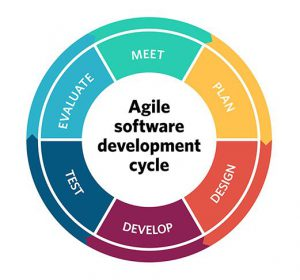
\includegraphics[width=10cm, height=9cm]{agile.jpg}
        \caption{The Agile Development Cycle. Adapted from \cite{1}.}
        \label{fig:mesh1}
    \end{figure}
\end{center}

We will be implementing an Agile development cycle for our project, as displayed above in  figure \ref{fig:mesh1}. This methodology emphasizes an active and collaborative approach to the software development life cycle. It involves designing, creating, and testing multiple iterations of the program and constantly evaluating its state with our client. Certain aspects of Agile development include gradual modifications to requirements, incremental versions of the program, frequent deliveries on products, integrated testing, and constant collaboration with stakeholders \cite{1}. We chose this development cycle to preemptively prepare for possible situations where we find that one design works better than another. The ability to change our direction to what would produce the best, most viable training module is a tremendous benefit that could assist in the probability of our success. While some aspects of the Waterfall methodology (which emphasizes a sequential progress flow) should be considered, such as adhering to overarching requirements and the general design format that our client would like to see in addition to comprehensive documentation, having the flexibility of Agile development will allow us to build a product that the client will more likely approve of.  

\section{Design description information content}
\subsection{Introduction}
This section will contain the following: an identification of the software design descriptions, identified design stakeholders, identified design concerns, selected design viewpoints, design views, design overlays, and design rationale.

\subsection{SDD identification}
In order to substantiate and validate our progress, the performance metrics established in our Problem Statement document will be addressed. The performance metrics specify certain aspects of our project that we will strive to complete. At several points in our project's duration, we will measure our progress based on the metrics below:

\begin{enumerate}
\item A VR environment is constructed with a PageWide Web Press in the scene. This environment should include recognizable graphics, sounds, and appear to represent a real world work environment to a reasonable extent.

\item The user can move around within the scene using the provided VR headset, and the user can interact with the press in at least one way using the provided controllers. 

\item The interactive parts of the VR press simulate at least one major function in virtual reality that would be covered in the physical reality training. Instructions should be given to the user with in-game audio and visual cues.  

\item The virtual reality press simulates failure when the VR press is operated incorrectly (controls used in the wrong order) in at least one (ideally all) of the functions in the training.

\item Outside individuals with no prior knowledge can complete the training successfully, without triggering a failure (when allowed repeat attempts), using only the instructions and prompts within the VR simulation. 

\item Positive user feedback on interaction and intuitive gameplay mechanisms, especially for users with no background in virtual reality or gaming controls in general.

\item Framework that can be used to easily implement future training scenarios after completion of capstone.

\item After completing the VR training program, users can correctly identify parts and functions of the real press that were covered in the program.
\end{enumerate}

The basis of our verification will be predicated on HP's evaluation of our performance. The performance metrics will prove to be useful as specific goals to strive for, but ultimately, HP and our client will determine the validity of our project. 

\subsection{Design stakeholders and their concerns}
Because of the fluid circumstances of our project, our client, Tim Holt, has defined our project goal to be that of a self-encapsulated program that contains a basic training module. An important aspect to our relationship with our stakeholder would be consistent interaction through weekly meetings in order to ensure that we are on the right track. Because of the limited time we have to develop the program, it is imperative that we actively ask questions and review our progress with our client on a regular basis. 
\subsection{Design views}
The main assumption in this document is that the contents of the training exercises/scenarios will be determined by HP during design planning meetings with Tim Holt, the project sponsor as development starts. We have not yet received technical manuals or descriptions of existing training seminars and as such have not been able to go through the these materials to gain an understanding of the contents of the scenarios.
\subsection{Design viewpoints}
At the conclusion of our project, we will have created training modules capable of being used with a correctly configured, mid-tier laptop and an HP Mixed Reality Headset. Resources include the CAD files and programs used to implement the modules. The program must be capable of being shared across physical distances so personnel can use it remotely. The documentation and instructions must also be clear and concise. For verification purposes, the personnel running the training modules can provide feedback in addition to any leadership supervising the training for the Web Press systems. One contingency to note is the demand for these training modules; if we had a limited number of personnel to train for the first time, we might not be able to receive enough feedback to properly make a case for the advancement of VR training for HP Web Press systems. 
\newpage

\subsection{Design elements}
% Design Entities
The following is a list of design entities with a description of their attributes, which include name, type, and purpose:

\begin{itemize}
    \item Name: Unreal Engine\\
          Type: Framework / Engine\\
          Description: A 3D engine from which we will build our application 
    \item Name: Blueprints\\
          Type: Generic templates\\
          Description: A set of functions in Unreal Engine to be used for visual scripting to reduce programming time
    \item Name: Sandbox Mode\\
          Type: Module\\
          Description: A portion of the program designed to allow users to freely interact with the 3D environment in an undirected setting 
    \item Name: Training Mode\\
          Type: Module\\
          Description: A portion of the program designed to allow users to be given a set of instructions that they must follow to complete some task
    \item Name: Player Controller\\
          Type: Component\\
          Description: A component which will allow the user to interact with the 3D environment, receiving input from a virtual reality headset and pair of controllers
\end{itemize}

\subsection{Design overlays}
% Business Analysis
Although we will have definitive methods with which to analyze the development of our modules, we will also begin the verification process during the business analysis portion of our project as well. Our design will require an extensive amount of verification as well in order to create as optimal and accurate a module as we can. Within our business analysis, we will be gathering data from previous virtual reality studies, instruction manuals, current training programs, and other resources to assist in the design of our modules. We will need to verify our design in terms of our use cases during every step of development. We will also speak with personnel involved with training in order to support our design plan for each module that we will strive to create. 

% Code/Documentation Sharing and Accountability
The management of our documentation, assignment submissions, code, CAD models, audio and video, notes, photos, and version control repositories will be a major factor that could allow us to provide a quantifiable measure with the resources we are developing. Software we will use will be Google Drive, Overleaf, and Github to share our code and documents. Verification will also involve monitoring the progress of each of our team members. By keeping each other accountable in the development of our tangible progress, we can strive for the optimization of a better product. 

% Talking with client
Among our requirements will be to regularly hold meetings with our client and be in constant discussion about our progress. We will be holding weekly meetings either at HP or on campus with our group and our client where we will go over our recent development and state our goals for the week. We will also document our progress on our individual class blog as well as within an informal work log. Emails will also be used to coordinate between our client throughout the week. In terms of our group dynamic, we will be communicating most often using Slack. In addition, we will also hold weekly meetings with our TA, Christopher Kawell for the class, updating him on our progress both as a group and individually. These meetings will be held in a scrum format where we will discuss what we've done and what we are planning to do. 
\subsection{Design rationale}
Many components of our project, such as which VR headset to use, have been predetermined by our client and is only subject to change should we have a justifiable alternative that could prove to be more beneficial to HP. As such, we will be using the Mixed Reality Headsets manufactured by HP as our hardware. Software-wise, we are going to use the Unreal Engine as it contains many design components that we would like to use in order to create our modules. 

The management of our code and documentation will be done using the software described in the "Design overlays" section (Google Drive, Overleaf, and Github) due to each software's ease of access and applicability for each task. 

The metrics used in the "SDD identification" section were included as a means to outline the items we should strive to accomplish. While some of the items are general, some are specific so as to emphasize the importance in crafting a detailed simulation that can improve user experience. This will aid in HP's evaluation of our performance. 


\subsection{Design languages}
The design language we are choosing to take advantage of is one that is a feature of Unreal Engine, which is Blueprints Visual Scripting. This design language is a system in Unreal Engine that acts as a complete gameplay scripting system that is based on the concept of using a node-based interface to create gameplay elements in the Unreal Editor. It is used to define object-oriented classes or objects. The system will allow our designers to implement features that would normally require writing code, and so will cut back on total development time. Any features that do not have a Blueprint solution will be implemented via programming, but most of the basic functionality of our system will be created using this system.

\newpage

\section{Design viewpoints}
\subsection{Introduction}
This section will describe several design viewpoints. It will illustrate these viewpoints in terms of design language selections, relates design concerns with viewpoints, and establishes language neutral names for these viewpoints. 

\subsection{Context viewpoint}
The environmental conditions will cover room-space requirements and safety measures for user and equipment.

The training application will be designed for room-scale VR with 3x3 meter available space in mind. Less space would still function well, but will allow for less physical user motion, such as stepping forward, leaning, turning, and stretching arms. 

The following simple protocols to setup the room environment will ensure safety of equipment and the user:
\begin{enumerate}
    \item Clean surrounding areas of all objects
    \item Ensure cables are not twisted
    \item Use the controller wrist straps
    \item Understand user's physical boundaries
\end{enumerate}
\subsection{Composition viewpoint}
The user will interface with the training program through a virtual reality headset. There are 2 main types of virtual reality headsets; built in motion camera headsets and external camera headsets. While the primary headset for the program will be a built in motion camera headset, Microsoft Mixed Reality, the training program will be equally compatible for both types of headsets.

External camera headsets use 1 or more cameras placed away from the headset. The field of view created by the camera(s) is the area that the headset and controllers can be moved within. With a built in motion camera headset, there is only 1 camera, built into the headset itself, and its forward facing field of view is the area the controllers can be moved within. Both have their own flaws. With the former, the headset can not move outside the play area, leaving the in game avatar stuck in place. With the latter, the controllers must be in front of the user, if the user tried to place their controllers above their head or behind them the controllers would become stuck at the edge of the viewport. 

The training program will use standard interface mechanics and inputs to guarantee cross compatibility with other forms of virtual reality headsets. Specifically, the program will highlight objects that can be interacted with, and will present button prompts to show which button is used to interact with the object.  

The VR application will be built for windows 10 systems, knowing that the primary headset will be HP's Windows Mixed Reality headset. No other third party software will be needed. This includes distribution software such as Steam.
\subsection{Logical viewpoint}

The training program will be structured as a series of menus presented to the user. These menus will control which of the training modes and scenarios are presented to the user for completion. Figure \ref{fig:logic_uml} describes the flow of logic through the menus and selecting the training mode, with stop conditions for each state. The training program will be structured in the form of a modern video game. Users will be given scenarios to perform and must complete the requirements of said scenario in order to pass and receive qualification. These qualifications will be stored on a per-user basis to prove to the proctor that the user has indeed passed the training.

\begin{center}
    \begin{figure}[h]
        \centering
        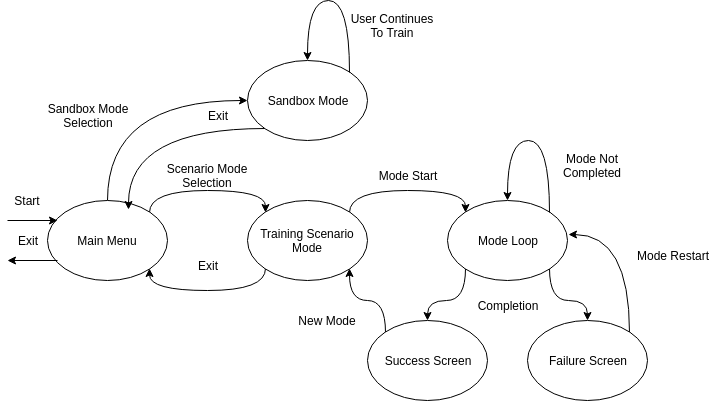
\includegraphics[width=15cm, height=9cm]{logical_view1.png}
        \caption{UML Diagram for the logic flow of the training program.}
        \label{fig:logic_uml}
    \end{figure}
\end{center}

\subsection{Dependency viewpoint}
The training program must contain a 3D recreation of the real HP Web Press in order to provide the most accurate training possible to the user. As much as possible, the program must behave in the same way as a real Web Press. HP will provide high quality 3D computer aided design files that can be imported into the Unreal Engine for our use.

Unfortunately, these CAD file might prove to be too detailed for our programs use. The goal is to have a training program that can be run on a middle tier priced laptop, and if the CAD files are too large in file size and detail it will cause the laptop to not be able to run the program at the desired frame rate.

In this event, we will redesign the CAD files to a more simple design to allow for the program to run at a smooth and stable frame rate.
\subsection{Information viewpoint}
There are only a few cases in which information is being managed for the user:
\begin{enumerate}
    \item Saving user scores
    \item Saving users records of completed training
    \item Saving user preferences
\end{enumerate}
All data will be stored locally on the machine the game is played on. No data is sent to or retrieved from the internet after the application has been installed. 

% Data Gathering and Analysis
After we develop our modules to the extent where we can begin user testing, we will want to quantify our project's performance by gathering data to analyze. As the purpose of our modules will be to train individuals on how to operate Web Press technology and based on our defined performance metrics, we will utilize the following to analyze our effectiveness: 
\begin{enumerate}
    \item User Feedback
    \item Efficiency in performing certain tasks
    \item Ability to implement new training scenarios
\end{enumerate}
Testing the system interface will be fully dependant on user feedback. We can develop objectives for the user to complete, such as mundane tasks like picking up objects and dropping them, to more complex scenarios. Feedback on interfaces will be based on a criteria of topics with questions pertaining to each. Questions will include asking how intuitive the task feels with little to no instructions, how responsive actions are, tester likes and dislikes about the functionality of in-game actions, and suggestions on what testers think they could benefit from.

Testing will involve the creating an user-name and completing training, while closing the game between each completion to ensure the data is been saved and loaded properly. To test the saving of user preferences the preference will need to be changed and the game will need to be reset to verify changes.

\subsection{Policies and regulations}
Policy will be dictated by HP. This system will belong to them as a HP licensed product. We as a development team will own no rights.

Official HP resources will be made available to this team under a non-disclosure agreement. These reference materials are not to be used in the final product, and instead are to be used in the creation of derivative models and works that will not fall under the non-disclosure agreement. The final program will be freely available to be shown off at the OSU Engineering Expo as part of the senior project capstone class.

\subsection{Interface viewpoint}
% User interfaces
The user interfaces of the software product necessary to accomplish the software requirements include a virtual reality display of 3D environments, a navigation interface for users to move through a 3D space, and text UI elements to allow a user to access information in the application. It is important that the software product is comfortable and understandable for users. Virtual reality can adversely effect users who are sensitive to motion sickness, so a consistent frame rate in the application is important for user comfort. Users must also be able to understand their environment and clearly see what options are available to them, such as where they are able to move and what they are able to interact with.

\subsection{Interaction viewpoint}
The training program should be accessible to everyone. No prior virtual reality or video gaming experience should be necessary to complete the training exercises provided by the program.

One of the biggest steps taken to keep the training program approachable will be the availability of different movement options for the user. The most common movement style in a typical VR game is teleportation: the user holds on button down on the controller and an indicator appears pointing to the location the user will be teleported to if they press another button. The user may move the pointer to a new location by moving the controller around in the virtual space, or they may cancel the movement command with a button press. Of course, the user will be able to physically walk around the real world and observe the same movement in the virtual world, but teleportation allows the user to have free reign of movement throughout the entire virtual space and not be limited to the dimensions of the physical surroundings.

Additionally, the user will be able to move around with the traditional gaming style of pointing the analog stick in the direction they want to move. This option will have to be opted into by users as the consensus of virtual reality players is that movement in this manner tricks their eyes into believing that there is actually physical motion occurring without movement from the legs, which has a high percent chance to cause nausea.

%Move this? ---> is this true?
% this should still be true. -nick
After the user completes a scenario or section of scenarios they must take a quiz about what they just accomplished. If they do not meet an information retention rate of at least 90\% they must complete the scenario or section of scenarios again until they are ale to achieve 90\% retention or better.

Additionally, some scenarios may be time dependant and require the user to finish the scenario requirements in the allotted time. If they do not complete the scenarios in the allotted time the scenario is marked as failed and the user must attempt that scenario again before they are allowed to take that scenario or scenario section quiz and move on to different scenarios.
\subsection{State dynamics viewpoint}
The training program will have two modes: scenario and sandbox.

Scenario mode puts the user into a predetermined event or series of events and requires them to participate until the desired outcome is achieved, or other limitations like a time limit runs out. For instance, one such scenario would be if the Web Press breaks down or has stopped printing the user must investigate the problem and return the press to a nominally functioning state. A subsection of the scenario mode will be the alarm gauntlet: a series of scenarios designed to test the users knowledge of the Web Presses many alarm systems and how to silence them by fixing the associated fault.

Sandbox mode is more free form. There is no time limit or overarching goal to achieve. Sandbox mode allows the user to interact with the Web Press as if they were standing next to a real one in person. The user may practice any feature of the Web Press they desire and the Web Press will respond as expected. Sandbox mode allows for user to test things they might not get to test on the real Web Press such as what happens if the Web Press's paper feeder jams and is not fixed in the proper amount of time, and what happens to the rest of the system as a consequence.

The significance of having both modes available allows personnel to first be trained to be trainable (via the sandbox mode) by familiarizing themselves with both Web Press and VR concepts. This invites them to succeed. Scenario mode, however, will teach the user how to deal with specific events, providing them with practical experience and can be more valuable in than sandbox mode in that it prepares the user how to handle such events, such as the Web Press breaking down. To justify and validate the use of two modes, user feedback will be gathered by HP personnel to inquire on the effectiveness of having scenario and sandbox mode.

\subsection{Algorithm viewpoint}
The goal will be to have four separate controller classes; Player controller, Quest-State Controller, UI controller, and Object Controller. From a high level viewpoint, each controller will use a modular class based design to allow expansion of features and modifications based on specific level design.

Each controller will be in charge of a different portion of user interaction and feedback, while also working together to provide a full experience.

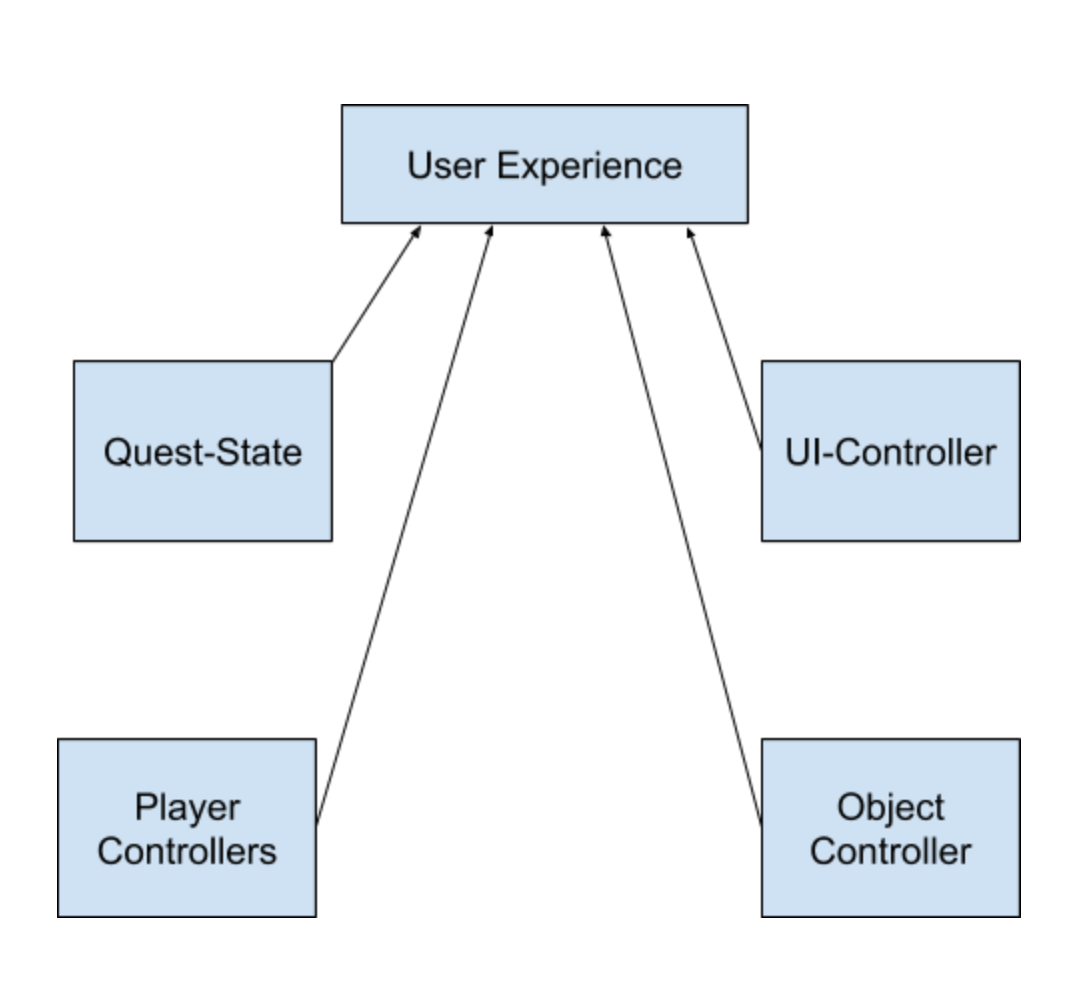
\includegraphics[width=200pt]{AlgoDia.png}

\subsubsection{Player Controller}
The Player Controller will be in charge primarily of player input and translating that information into the virtual world. The Player Controller will also be in charge of all variables related to the player, such as player scores.
\subsubsection{Quest-State Controller}
The Quest-State Controller is in charge of all task oriented logic and the current state of the quest events.
\subsubsection{UI Controller}
The UI Controller will be managing all UI displayed to the user on screen. This includes touchable floating text, buttons, and scores. The variables for these variables will be referenced from the Player and Quest-State Controller.
\subsubsection{Object Controller}
The Object Controller class will be what all non player objects inherit, such as interactive objects. This will be in-charge of when an object can be initialized or destroyed, and whether or not it contains physical properties or other unique characteristics.

\subsection{Resources viewpoint}
Since this program will be run as an Unreal Application on internal company servers and computers, security will not be a major focus. Our team does understand that some printer models will not be of public knowledge (secret), so any public demo will use only public printer models.

As far as data security is concerned, all files will be built and compiled using Unreal for internal use only. We will not be implementing any method to protect assets, such as CAD models, from being stolen from the company's internal servers.
\appendices
%\section{Bibliography}
\begin{thebibliography}{}
\bibitem{1}
Project-Management, “10 Key Principles of Agile Software Development,” Best Project Management Software Reviews, Oct. 8, 2018. [Online]. Available: https://project-management.com/10-key-principles-of-agile-software-development/ [Accessed: Nov. 27, 2018].


\end{thebibliography}

%\section{Conforming design language description}

%\section{Templates for an SDD}






\end{document}

